% !TEX root = ../../main.tex

\section{Résultats numériques des schémas de Lawson approchés}
% -------------------------------------------------------------------
\label{s:3:num_m}

Dans cette section nous effectuerons une comparaison entre les résultats obtenus la section~\ref{sec:3:num} avec une méthode de Lawson où la résolution de la partie linéaire est exacte mais ne contient pas les équations de Maxwell, et la méthode proposée dans la section~\ref{s3:approx} avec une approximation de la partie linéaire, permettant de prendre en compte plus de termes au sein de celle-ci. L'utilisation de troncatures de la série de Taylor, ou d'approximants de Padé, permet toujours d'effectuer le filtrage de l'équation de Vlasov effectué dans la sous-section~\ref{ssec:3:filtrage}.

La condition initiale est choisie de la même manière que précédemment, c'est-à-dire conformément à~\cite{Holderied:2020}, qui est une distribution maxwellienne anisotrope, qui mène à une instabilité de type Weibel :
$$
  f_h(t=0,z,\vb{v}) = \frac{\rho_h}{(2\pi)^{3/2}\bar{v}_{\|}\bar{v}_\perp^2}\exp( - \frac{v_z^2}{2\bar{v}_{\|}^2} - \frac{\left( v_x^2 + v_y^2 \right)^2}{2\bar{v}_\perp^2} )
$$
avec $z\in[0,\frac{2\pi}{k}]$, $k=2$, $\bar{v}_{\|}=0.2$, $\bar{v}_\perp=0.6$, $\rho_h=0.2$ et $B_x(t=0,z)=\epsilon\sin(kz)$. Les autres inconnues du système $(j_{c,x},j_{c,y},B_y,E_x,E_y)$ sont initialisées à zéro. Le domaine en vitesse est restreint à $\vb{v}=(v_x,v_y,v_z)\in[-3.6,3.6]\times[-3.6,3.6]\times[-2.4,2.4]$ et on note $N_z$, $N_{v_x}$, $N_{v_y}$, $N_{v_z}$ le nombre de points de discrétisation dans chaque direction.

Dans les diagnostics que nous allons présenter, nous regardons les mêmes quantités, à savoir les énergies magnétiques, électriques et l'énergie cinétique des particules froides, décrites dans les équations~\eqref{eq:3:nrj:me}-\eqref{eq:3:nrj:ce}, ainsi que la préservation de l'énergie totale. Les seuls solveurs que nous étudions dans cette section sont des méthodes de Lawson induites par les méthodes RK(3,3) de Shu-Osher ou RK(4,4), où l'exponentielle la partie linéaire, $e^{\Delta tL}$, sera approchée par une troncature de la série de Taylor ou un approximant de Padé à différents ordres.

%La génération de code, discutée dans la section~\ref{ssec:3:codegen}, a été intensément utilisée dans cette section, et a permis l'implémentation efficace de ces méthodes. Des conflits de versions de compilateurs ont imposé l'exécution du code de calcul sur une autre grappe de calcul que celle utilisée précédemment.

\subsection{Comparaison des troncatures à pas de temps constant}

Dans un premier temps nous souhaitons étudier la faisabilité de ne pas résoudre exactement la partie linéaire d'une méthode de Lawson. Pour cela nous conservons la partie linéaire~\eqref{eq:3:LNsmaxwell}, déjà utilisée dans les premiers résultats dans la section~\ref{sec:3:num} et étudions l'impact sur les résultats avec les mêmes paramètres numériques, en particulier le pas de temps $\Delta t=0.05$, et une méthode d'approximation d'ordre supérieur à la méthode de Lawson LRK(4,4) utilisée, à savoir $T_5$ et $P_{2,2}$. Ces résultats sont observables sur les trois énergies sur la figure~\ref{fig:approx:energies4d}. Les résultats coïncident parfaitement avec les résultats précédents, ce qui permet de confirmer la faisabilité de construire une méthode de Lawson avec une partie linéaire approchée qui contient les équations de Maxwell.

\begin{figure}[h]
  \centering
  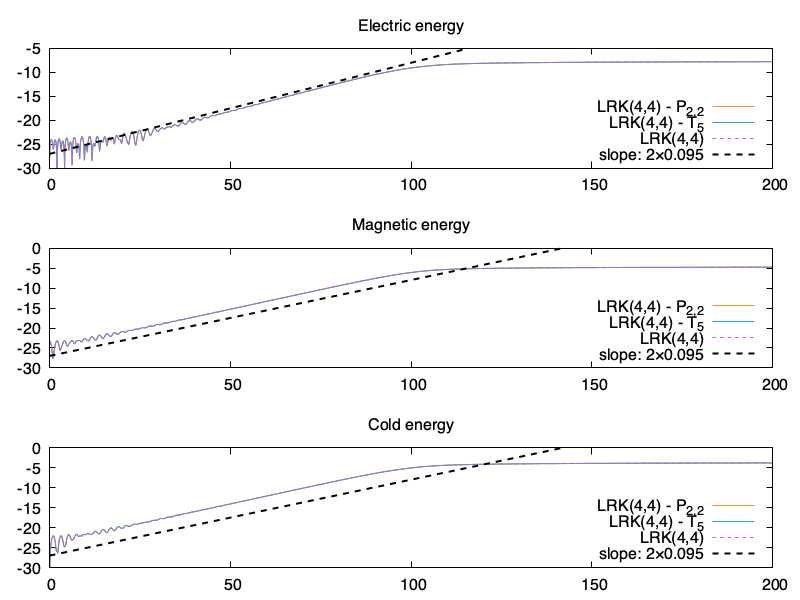
\includegraphics[width=0.9\textwidth]{\localPath/figures/energy_verif.png}
  \caption{Évolution de l'énergie électrique, magnétique et l'énergie cinétique des particules froides définies dans les équations~\ref{eq:3:nrj:me}-\ref{eq:3:nrj:ce}, en échelle semi-$\log$, pour les méthodes de Lawson LRK(4,4) classique, avec troncature de la série de Taylor à l'ordre 5 ($T_5$), et approximant de Padé d'ordre $(2,2)$ ($P_{2,2}$). $\Delta t = 0.05, N_x=27, N_{v_x}=32, N_{v_y}=32, N_{v_z}=41$.}
  \label{fig:approx:energies4d}
\end{figure}

Sur la figure~\ref{fig:approx:energies:cfl} on effectue la comparaison entre une méthode de Lawson approchée avec la partie linéaire donnée par~\eqref{eq:3:LNsmaxwell} (test précédent) et avec la partie linéaire donnée par~\eqref{eq:3:LNmaxwell}, présentées dans la section~\ref{s3:approx}, avec un pas de temps $\Delta t=0.12$ supérieur à l'estimation de stabilité faite dans la section~\ref{ssec:3:cflMaxwell} sur la résolution explicite des équations de Maxwell. On remarque l'intérêt d'intégrer les équations de Maxwell dans la partie linéaire (courbes étiquetées \emph{Maxwell inside}) où le schéma est stable, les simulations effectuées avec la partie linéaire précédemment utilisées sont instables car la contrainte de stabilité est violée. L'absence de condition de stabilité provenant des équations de Maxwell permet de prendre des pas de temps plus grand. Cependant il reste une condition de stabilité provenant du transport non-linéaire $(\vb{E}+\vb{v}\times\vb{B})\cdot\nabla_{\vb{v}}f_h$. Il est étonnant que les simulations mettant en jeu la troncature de la série de Taylor fonctionnent aussi bien au vu des résultats précédents de la section~\ref{s3:approx}, cela peut venir de l'absence de hauts modes de Fourier dans la simulation.

\begin{figure}[h]
  \centering
  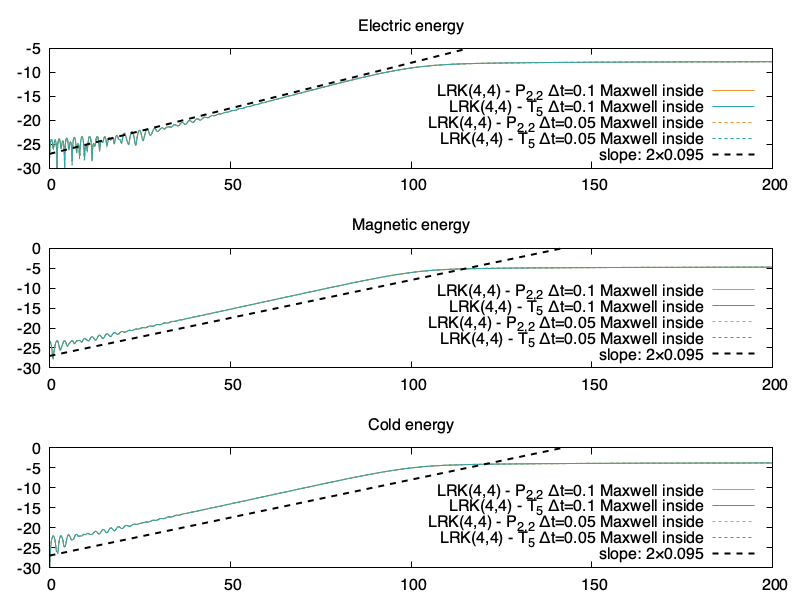
\includegraphics[width=0.9\textwidth]{\localPath/figures/energy_max.png}
  \caption{Évolution de l'énergie électrique, magnétique et l'énergie cinétique des particules froides définies dans les équations~\ref{eq:3:nrj:me}-\ref{eq:3:nrj:ce}, en échelle semi-$\log$, pour les méthodes de Lawson LRK(4,4) classique, avec troncature de la série de Taylor à l'ordre 5 $T_5$, et approximant de Padé d'ordre $(2,2)$ $P_{2,2}$. $\Delta t = 0.12, N_x=27, N_{v_x}=32, N_{v_y}=32, N_{v_z}=41$.}
  \label{fig:approx:energies:cfl}
\end{figure}

Nous étudions maintenant l'influence sur les résultats de différents approximants de Padé. En particulier nous testons des ordres inférieurs à la méthode de Lawson, ainsi que des approximants de Padé avec des degrés différents pour le numérateur et le dénominateur ($P_{1,2}$ et $P_{2,1}$). On remarque sur la figure~\ref{fig:approx:energies:pade} que l'on a une très bonne correspondance dans les résultats entre les différents approximants de Padé, les résultats précédents, et les relations de dispersion. Il n'y a que le cas où le degré du numérateur est supérieur au dénominateur, $P_{2,1}$, que le schéma est instable, comme prédit par la figure~\ref{fig:ev:P21}.

\begin{figure}[h]
  \centering
  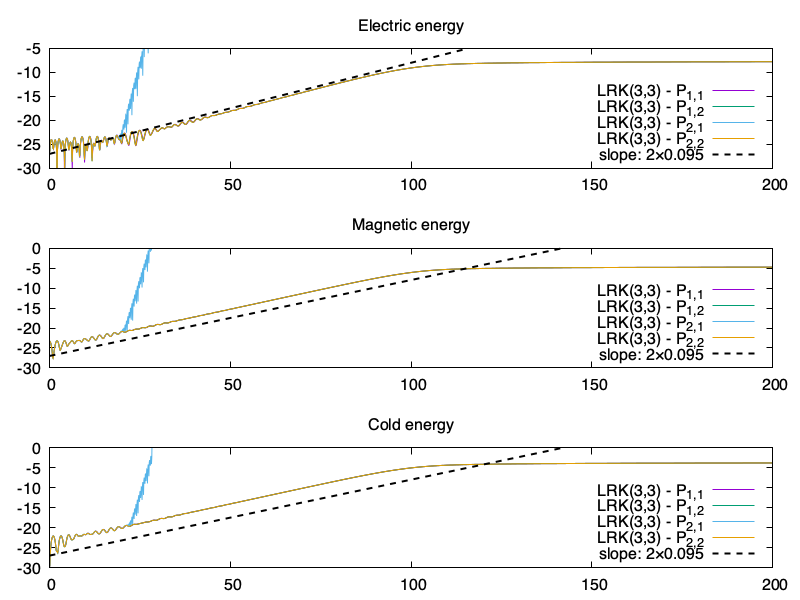
\includegraphics[width=0.9\textwidth]{\localPath/figures/energy_pade.png}
  \caption{Évolution de l'énergie électrique, magnétique et l'énergie cinétique des particules froides définies dans les équations~\ref{eq:3:nrj:me}-\ref{eq:3:nrj:ce}, en échelle semi-$\log$, pour les méthodes de Lawson LRK(3,3) de Shu-Osher, avec différents approximant de Padé d'ordre $(1,1)$, $(1,2)$, $(2,1)$ et $(2,2)$. $\Delta t = 0.1, N_x=27, N_{v_x}=32, N_{v_y}=32, N_{v_z}=41$.}
  \label{fig:approx:energies:pade}
\end{figure}

%%%%%%%%%%%%%%%%%%%%%%%%%%%%%%%%%%%%%%%%%%%%%%%%%%%%%%%%%%%%%%%%%%%%%

\FloatBarrier
\subsection{Étude à pas de temps adaptatif}
% -------------------------------------------------------------------

L'intérêt principal d'intégrer les équations de Maxwell dans la partie linéaire de la méthode de Lawson est de pouvoir satisfaire le point \ref{list:ii} présenté dans la section~\ref{ssec:3:dtn}, c'est-à-dire ne pas avoir de contrainte de stabilité trop forte provenant des équations de Maxwell. Une fois affranchi de ce point, la méthode de pas de temps adaptatif LDP4(3) peut sélectionner des pas de temps plus important en théorie. Le calcul des pas de temps s'effectue sans limiteur :
$$
  \Delta t_0 = 0.1,\quad \Delta t_{n+1} = \sqrt[p]{\frac{tol}{L_{[p]}^{n+1}}}\Delta t_n\ ,n\geq 0
$$
où $L_{[p]}^{n+1}$ est l'erreur locale calculée par~\ref{eq:Lerror}, $p=4$ représente l'ordre maximal du schéma en temps, le choix du pas de temps initial est simplement dicté par les tests précédents.

La figure~\ref{fig:approx:energies:dtn} montre les différentes énergies en échelle semi-log. On retrouve avec les deux méthodes, troncature de la série de Taylor et approximant de Padé, le bon taux d'instabilité et la saturation s'effectue au même niveau d'énergie. Il existe un décalage dans les résultats dû aux grands pas de temps calculés initialement par la méthode de Lawson couplé à un approximant de Padé, celui-ci peut-être corrigé par un limiteur comme dans la section~\ref{ssec:3:dtn}. En effet, la figure~\ref{fig:approx:iterations:dtn} retrace l'historique du pas de temps au cours des itérations, et seule la méthode couplée à un approximant de Padé sélectionne de grands pas de temps (supérieur à 1) pendant la phase linéaire. Durant cette phase, les champs électromagnétiques $(\vb{E},\vb{B})$ sont très faible et la contrainte de stabilité du terme non-linéaire est donc très peu restrictive. On trouve ici tout l'intérêt de ces schémas, la partie linéaire est résolue exactement pour tout pas de temps $\Delta t$ ; lorsque lorsque les effets non-linéaires, qui imposent une condition de stabilité, deviennent important des petits pas de temps sont pris automatiquement pour capturer la dynamique complexe non-linéaire. La restriction à de petits pas de temps avec la troncature de Taylor peut s'expliquer par le fait que la méthode est instable théoriquement d'après l'étude des valeurs propres faites précédemment. La méthode LDP4(3) couplée à $P_{2,2}$ permet l'usage de grands pas de temps, on observe bien la phase linéaire (jusqu'au temps $t\approx 100$) où les champs électromagnétiques sont encore faibles et la stabilité n'est pas contrainte par les termes non-linéaires du transport en $v$. Après cela, dans la phase non-linéaire, le pas de temps décroit et se stabilise autour de $\Delta t\approx 0.19$ (contre une stabilisation autour de $\Delta t\approx 0.11$ pour la méthode couplée à $T_5$). La section du bas de la figure~\ref{fig:approx:iterations:dtn} retrace l'évolution de l'erreur locale pour toute les itérations, les itérations rejetées par le critère d'erreur sont représentées par des carrés. On observe, comme dans les précédents cas tests sans les équations de Maxwell dans la partie linéaire sur la figure~\ref{fig:dtanderrordp43} de la section~\ref{ssec:3:dtn}, un grand nombre d'itérations rejetées. Ce phénomène entraine un surcoût supplémentaire qui pénalise la méthode de Lawson couplée avec la troncature de la série de Taylor, en effet la simulation avec un pas de temps constant $\Delta t=0.12$ à un temps de calcul de 5h58, temps passant à 6h27 avec la méthode à pas de temps adaptatif. La stratégie basée sur un approximant de Padé propose quant à elle des temps de calcul de 5h59 avec un pas de temps constant $\Delta t=0.12$ (pas de surcoût observé entre la série de Taylor et l'approximant de Padé), et un temps de 3h49 pour la méthode à pas de temps adaptatif.

\begin{figure}[h]
  \centering
  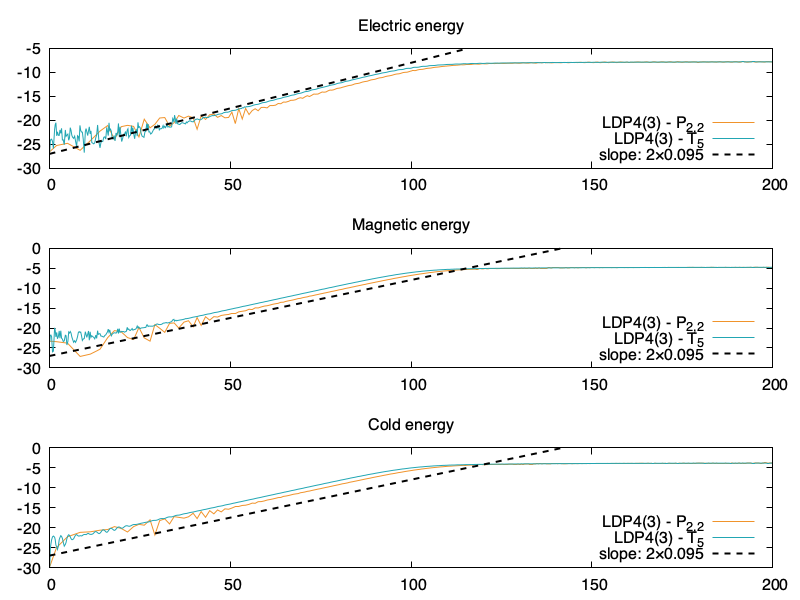
\includegraphics[width=0.9\textwidth]{\localPath/figures/energy_dtn.png}
  \caption{Évolution de l'énergie électrique, magnétique et l'énergie cinétique des particules froides définies dans les équations~\ref{eq:3:nrj:me}-\ref{eq:3:nrj:ce}, en échelle semi-$\log$, pour les méthodes de Lawson LRK(4,4) avec troncature de la série de Taylor à l'ordre 5 $T_5$, et approximant de Padé d'ordre $(2,2)$ $P_{2,2}$. $\Delta t_0 = 0.1, N_x=27, N_{v_x}=32, N_{v_y}=32, N_{v_z}=41$.}
  \label{fig:approx:energies:dtn}
\end{figure}

\begin{figure}[h]
  \centering
  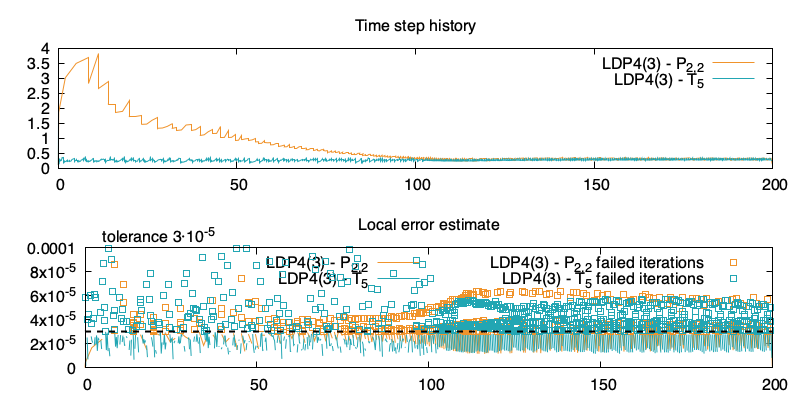
\includegraphics[width=0.9\textwidth]{\localPath/figures/iterations_dtn.png}
  \caption{Évolution du pas de temps au cours du temps (haut) et de l'estimation de l'erreur locale au cours du temps (bas), pour les méthodes de Lawson LRK(4,4) avec troncature de la série de Taylor à l'ordre 5 $T_5$, et approximant de Padé d'ordre $(2,2)$ $P_{2,2}$. $\Delta t_0 = 0.1, N_x=27, N_{v_x}=32, N_{v_y}=32, N_{v_z}=41$.}
  \label{fig:approx:iterations:dtn}
\end{figure}
